\documentclass[11pt]{article}
\usepackage[margin=0.85in]{geometry}
\usepackage{graphicx}
\usepackage{amsmath}
\title{R100: finite support of the marked-23 lambda norm}
\author{Koblitz modular IC research}
\date{3 November 2026}
\begin{document}
\maketitle
R99's degree-1968 norm numerator has 74 terms, all with exponents divisible
by 16. R100 verified that it is the sixteenth power of a degree-123
polynomial over $\mathbf F_2[x]$ and factored that root into irreducible
factors of degrees 11, 22, and 1, with respective exponents 1, 3, and 46.
The full factor product and a changed-product control passed. A fresh
Singular process reproduced the output byte for byte. An independent
Python GF(2) implementation checked the Frobenius identity, factor product,
and Rabin irreducibility of each factor. Lean 4.34.1 checked the degree
arithmetic.

\begin{center}
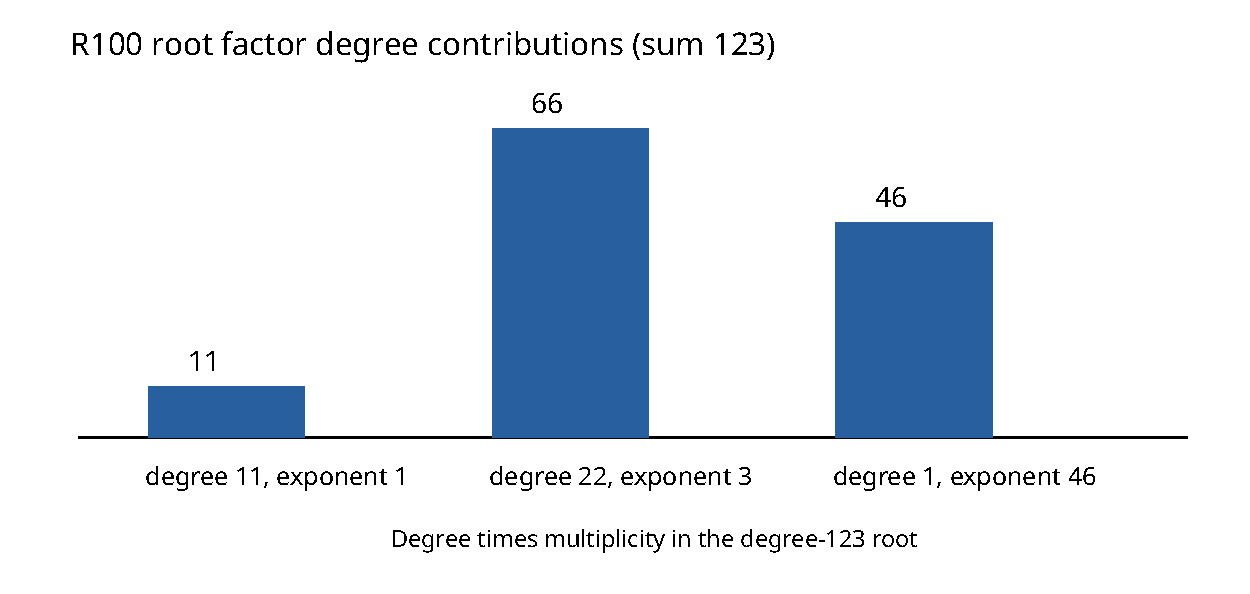
\includegraphics[width=0.93\linewidth]{diagram.pdf}
\end{center}

The finite zero support of this displayed lambda-order norm on $D(x)$ is
$x=1$ plus degree-11 and degree-22 closed points. Combining it with the
R97 base-order discriminant gives five finite supports to normalize:
$x=0$, $x=1$, and points of degrees 7, 11, and 22. Infinity is separate.
These factor exponents are not normalized ramification indices.

The first R100 preparation rejected its own off-by-one count: 73
positive-exponent terms plus constant 1 make 74. The failed preparation
was retained, R99's note and PDF corrected, and amendment 02 committed
before the accepted attempt. The raw archive SHA-256 is
\texttt{aff76c57c1a8213306d16bb6ea238f90704a576756eda54405e1419d7}\linebreak
\texttt{f20486b}.
\end{document}
